\documentclass{article}

% Use the neurips_2026 style file provided
\usepackage{neurips_2026}
\usepackage[utf8]{inputenc}
\usepackage[T1]{fontenc}
\usepackage{hyperref}
\usepackage{url}
\usepackage{booktabs}
\usepackage{amsfonts}
\usepackage{nicefrac}
\usepackage{microtype}
\usepackage{xcolor}
\usepackage{amsmath}
\usepackage{graphicx}
\usepackage{multirow}
\usepackage{tikz}
\usetikzlibrary{arrows.meta,shapes.geometric,shapes.symbols}


\title{Beyond the Next Token: Latent Execution-Graph Retrieval for Agentic Planning}

% \title{LEGR: Latent Execution-Graph Retrieval for Agentic Planning}
\author{%
  Tanay Kadam \\
  North Carolina State University, Lenovo \\
}

\begin{document}

\maketitle
\begin{abstract}
Routing natural-language requests to the appropriate tools, and multi-step tasks to the appropriate \emph{tool-execution graph}, remains a major bottleneck in agentic systems. Many existing approaches rely on coarse semantic taxonomies, which can degrade under query rephrasing, and can incur significant latency when they rely on multi-step autoregressive planning or cascaded tool selection. We propose two complementary methods for efficient and robust tool selection. First, we introduce a \emph{functional taxonomy} that groups tools by \emph{action type} rather than topic, improving routing accuracy by up to 18.5 percentage points under lexical variation. Second, instead of autoregressive planning, we introduce \textbf{Latent Execution-Graph Retrieval (LEGR)}, which retrieves an execution DAG from a pre-indexed corpus using a dual-encoder architecture. We train LEGR with a graph-aware contrastive objective regularized by graph edit distance to preserve workflow topology in latent space. On benchmarks derived from ToolBench and BFCL, LEGR achieves strong zero-shot generalization to held-out topologies with Recall@1 of 0.963 and reduces mean planning latency to 4.39\,ms, yielding a more than $400\times$ speedup over autoregressive LLM planners. Code and benchmark data are available at \href{https://github.com/tanay-kadam/LEGR}{LEGR}
\end{abstract}

\begin{figure*}[t]
\centering
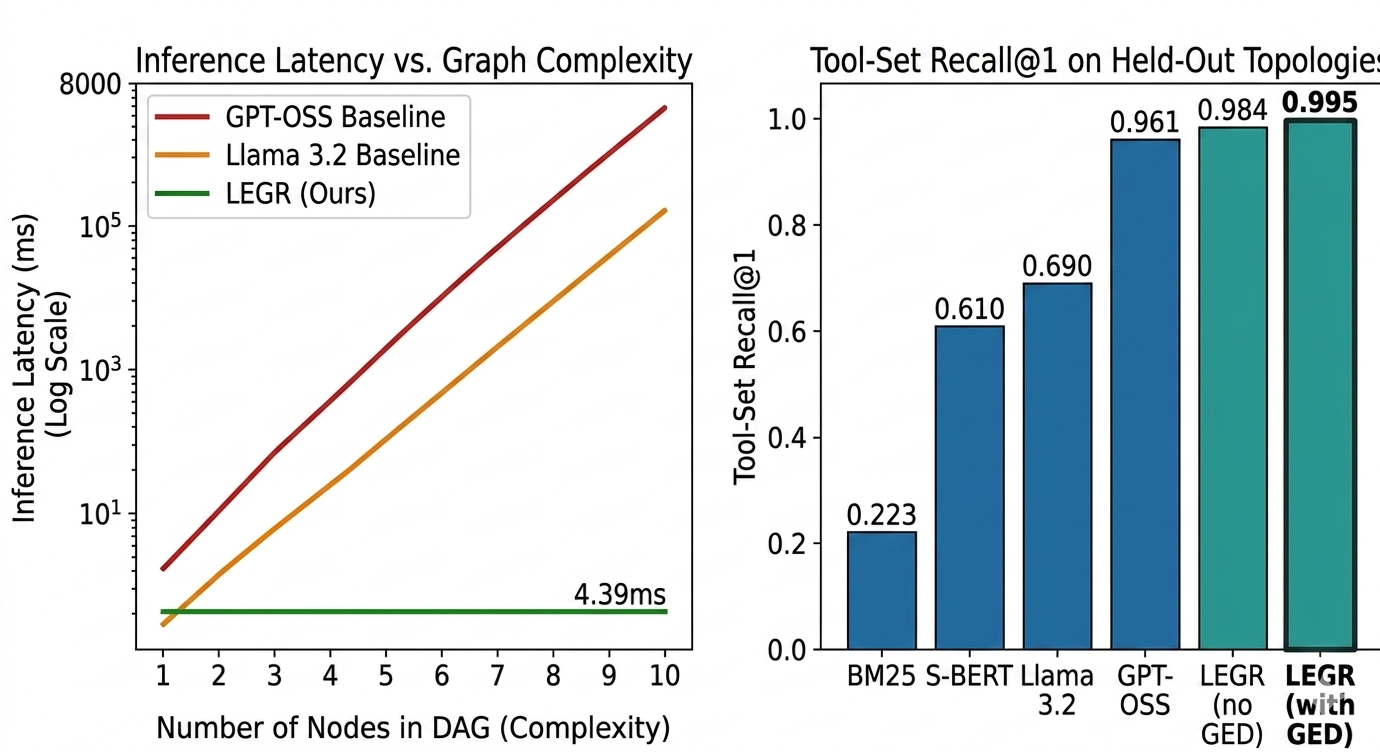
\includegraphics[width=\textwidth]{results.png}
\caption{\textbf{Core LEGR Results and Scalability Analysis.} \textbf{(Left) Inference Latency vs. Graph Complexity.} Autoregressive LLM baselines exhibit linear latency growth as the execution DAG grows (more tool nodes to describe). LEGR performs a single retrieval and remains constant at 4.39\,ms. \textbf{(Right) Retrieval Accuracy on Held-Out (OOD) Topologies.} Recall@1 comparison on the \textit{test\_topology\_heldout} split. LEGR outperforms lexical (BM25) and dense (S-BERT) baselines, and the GED-weighted loss further improves structural alignment.}
\label{fig:results}
\end{figure*}

\section{Introduction}

Tool-augmented LLM systems increasingly rely on an \emph{intent router}: given a user request, the router must select the appropriate tool(s) and, for multi-step tasks, a valid \emph{execution structure} (often a directed acyclic graph, DAG) that respects data and control dependencies across tool calls \cite{mialon2023augmented,shen2023hugginggpt,song2023restgpt}. For real-world AI assistants, this decision should not merely  be semantic. Selecting a ``nearby'' tool with the wrong action type (e.g., a write instead of a read) can create irreversible side effects, and emitting an incorrect dependency edge can silently corrupt downstream tool inputs.

In practice, intent routing  fails mainly for two reasons. \textbf{(1) Taxonomy mismatch:} many organize tools under human-friendly topic categories (e.g., HR vs. Finance). Topic labels are weak proxies for what a tool \emph{does}, especially when sibling tools share nouns but differ in side effects (read vs. write), scope, or safety constraints. As a result, routers overfit to topical keywords and become brittle under paraphrase, lexical variations, or ``confusable'' sibling tools. \textbf{(2) Autoregressive planning cost:} many planners ask an LLM to output an explicit textual serialization of a multi-step plan (tool names, arguments, and dependencies) token-by-token. Because decoding is sequential, latency grows linearly with the number of emitted plan tokens, which grows with workflow size and often adversely impacts responsiveness.

We address both issues with (i) a tool taxonomy based on function types (ii) a retrieval-based planner for multi-step execution trajectories. Concretely, we reorganize tool libraries around \emph{action types} and retrieve a pre-validated execution DAG instead of autoregressively generating next tools for the trajectory. This paper makes the following contributions:
\begin{itemize}
    \item We demonstrate that supervising intent routers with  \textbf{functional taxonomy} (grouping by action type rather than topic) improves routing accuracy by up to 18.5\% points under lexical variations.
    \item We introduce \textbf{Latent Execution-Graph Retrieval (LEGR)}, which frames multi-tool planning as dual-encoder retrieval of an execution DAG. This yields constant-time planning latency at inference (4.39\,ms, an over $400\times$ speedup compared to autoregressive LLMs, as shown in Figure~\ref{fig:results}).
    \item We propose a graph-aware training objective for LEGR: a contrastive loss regularized by Graph Edit Distance (GED) to encourage the latent space to respect workflow topology, not just semantic tool overlap.
    \item We release a benchmark for routing and execution-graph retrieval derived from ToolBench and BFCL, and show that LEGR generalizes zero-shot to held-out execution topologies (e.g., Diamond DAGs never seen during training) with a Recall@1 of 0.963.
\end{itemize}

\begin{figure*}[t]
\centering
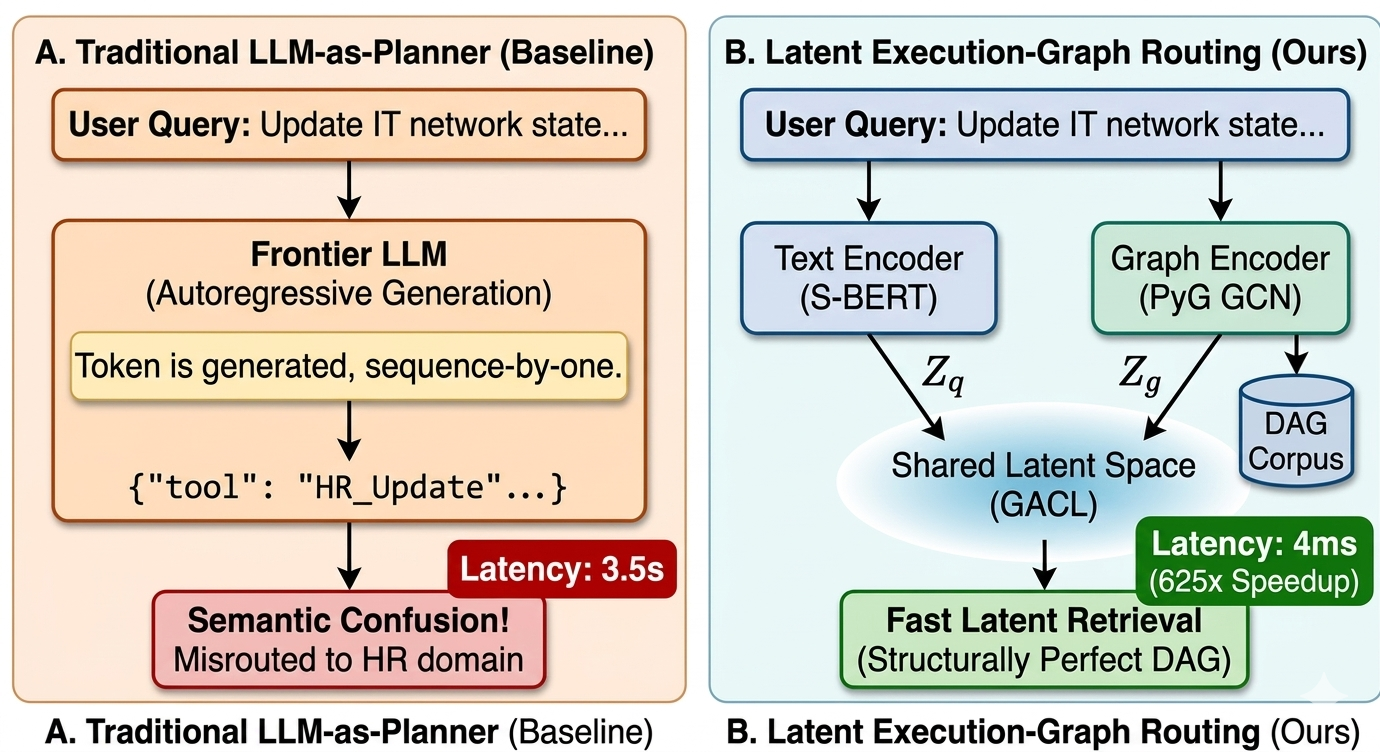
\includegraphics[width=\textwidth]{legr.png}
\caption{\textbf{Figure 1: Teaser.} Comparison between a traditional autoregressive LLM tool planner and our proposed Latent Execution-Graph Retrieval (LEGR). Left: token-level planning can topically drift and misroute requests to the wrong topic. Right: LEGR directly retrieves the correct execution DAG in a shared latent space, yielding much lower latency.}
\label{fig:teaser}
\end{figure*}

\section{Background and Related Work}

We have motivated two requirements for agentic tool use: routing decisions should reflect \emph{action types} (what actions a tool can execute), and multi-step plans should be produced with predictable, low latency. We review three relevant threads of work and highlight the specific gaps our work targets.

\textbf{Tool-augmented LLMs and taxonomy mismatch.}
Toolformer \cite{schick2023toolformer} and Gorilla \cite{patil2023gorilla} showed that LLMs can be trained to emit syntactically valid tool invocations, and benchmarks such as ToolBench \cite{qin2023toolllm}, BFCL \cite{yan2024berkeley}, and API-Bank \cite{li2023apibank} scaled evaluation to large API suites. Frameworks like AutoGen \cite{wu2023autogen} have further formalized how multiple agents and tools interact.
In many deployments, however, tool libraries are exposed through \emph{topic taxonomies} (e.g., HR, Finance, IT) because these are easy for humans to curate.
For routing, topic labels are neither necessary nor sufficient. For example, \texttt{Get\_Employee\_Record} (an idempotent read) and \texttt{Update\_Employee\_Record} (a state-changing write) share the same noun phrase but induce qualitatively different system-side effects.
Routers trained against topic branches are therefore incentivized to latch onto topical keywords, making them fragile under paraphrase, lexical variations, and ``confusable siblings'' that share nouns but differ in safety or idempotency constraints.
Our \textit{Functional Taxonomy} addresses this supervision mismatch by grouping tools by \emph{action class} (read, write, orchestrate), so the router is trained on the same decision boundary that governs system risk.

\textbf{Multi-step planning and the autoregressive bottleneck.}
Beyond selecting individual tools, agentic systems must often produce an \emph{execution structure} that captures dependencies among tool calls (e.g., a fan-out to parallel reads followed by a join).
A common approach is to serialize a workflow as text, often a JSON-like plan enumerating tool nodes, arguments, and edges, and have an LLM generate that serialization token-by-token.
Methods such as ReAct \cite{yao2023react}, Plan-and-Solve \cite{wang2023plan}, and LLM+P \cite{liu2023llmp} expand capability by increasing intermediate plan text, while ToT \cite{yao2023tree} and GoT \cite{besta2023graph} extend planning to tree/graph-structured search, and frameworks like DSPy \cite{khattab2023dspy} compile these steps into declarative pipelines.
The computational consequence is unavoidable: decoding $N$ output tokens requires $N$ sequential forward passes through the model, so planning latency scales as $\mathcal{O}(N)$ with the length of the emitted plan.
For non-trivial DAGs, $N$ grows with the number of nodes and edges that must be written down, producing multi-second delays in practice and additional overhead when the model self-corrects malformed plans.

\textbf{Retrieval-based tool use and topological blindness.}
To bypass the autoregressive bottleneck, one might look to retrieval-based methods. Retrieve-then-generate pipelines are standard for large tool libraries. Sparse retrievers (BM25) \cite{robertson2009probabilistic} and dense retrievers (Sentence-BERT, DPR) \cite{reimers-gurevych-2019-sentence,karpukhin2020dense} efficiently fetch relevant tool documentation or candidate APIs.
However, these retrievers typically treat candidates as \emph{flat text}, discarding the dependency structure that distinguishes ``the same tools in a chain'' from ``the same tools in a fan-out.''
Graph neural networks such as GCNs \cite{kipf2017semi} can encode structure, yet aligning natural-language intents with \emph{executable DAGs} (not just tool lists) remains underexplored.
LEGR targets this gap with a dual-encoder that maps queries and execution graphs into a shared space. By training with a contrastive objective regularized by Graph Edit Distance \cite{sanfeliu1983distance}, latent proximity reflects both tool overlap and workflow topology. This lets planning reduce to a single nearest-neighbor lookup rather than token-level synthesis.

\section{Methodology}

We propose a two-component framework for robust agentic intent routing: (1) a supervision scheme for \emph{which tool(s) to call} via \emph{Functional Taxonomies}, and (2) a retrieval-based planner, \textit{Latent Execution-Graph Retrieval} (LEGR), for \emph{how those calls are composed} into a multi-step workflow (an execution DAG).

\subsection{Problem Setup and Notation}
Let $q$ be a user request. Let $\mathcal{T}$ denote the tool library, and let $\mathcal{C} = \{\mathcal{G}_1,\dots,\mathcal{G}_{|\mathcal{C}|}\}$ be a corpus of \emph{candidate execution DAGs} curated offline. Each DAG $\mathcal{G}=(\mathcal{V},\mathcal{E})$ represents a valid multi-tool workflow, where nodes are tool invocations and edges encode data or control dependencies. The goal is to output a workflow $\hat{\mathcal{G}}$ that (i) calls the correct tools and (ii) matches the intended dependency structure.

A recurring source of brittleness in prior systems is that they often entangle two distinct design choices:
(i) \textbf{routing supervision}: the label space used to train the router to pick tools (i.e., the \emph{taxonomy}); and
(ii) \textbf{workflow planning}: the mechanism that constructs a multi-step execution structure (e.g., a tool chain vs. a fan-out DAG).
We address these separately. First, we define a taxonomy that better matches tool \emph{action types}. Second, we plan by retrieving an execution DAG.

\subsection{Functional vs. Topic-Based Taxonomies}
A \textbf{taxonomy} here simply means a partitioning of the tool library into routing labels used for supervision. We contrast two choices.

\textit{Semantic taxonomies} ($\mathcal{T}_s$) group tools by topical or organizational subject (e.g., HR, Finance, IT). This can collapse operationally different actions into the same branch. For example, \texttt{reset\_user\_password} (a credential \emph{write}) and \texttt{generate\_access\_report} (a read-only \emph{audit}) both fall under ``Identity Management.'' A router trained on $\mathcal{T}_s$ can therefore overfit to topic nouns (``access'', ``identity'') and become brittle under paraphrase, noun omission, or confusable wording.

We instead use a \textit{Functional Taxonomy} ($\mathcal{T}_f$), which groups tools by \textbf{action type} (the kind of external effect the tool can produce) so the supervision signal reflects the operational decision boundary. Concretely, we use three top-level action classes:
\begin{itemize}
    \item \textbf{State Modification:} state-changing tools (e.g., POST/PATCH requests, credential resets, record updates).
    \item \textbf{Data Retrieval:} idempotent, read-only tools (e.g., GET requests, audit queries, status checks).
    \item \textbf{Orchestration:} meta-tools that manage control flow (e.g., conditional branching, delegation).
\end{itemize}
Supervising the router under $\mathcal{T}_f$ reduces reliance on brittle topic vocabulary by emphasizing what the tool \emph{does} (read vs. write vs. control), not what the request \emph{talks about}.

\subsection{Latent Execution-Graph Retrieval (LEGR)}
LEGR replaces autoregressive plan synthesis with \emph{bi-encoder retrieval} in a shared latent space $\mathbb{R}^d$.

\textbf{Text encoder.} A Transformer encoder $f_\theta(\cdot)$ (\texttt{all-MiniLM-L6-v2}) maps the request $q$ to an embedding $\mathbf{z}_q \in \mathbb{R}^d$.

\textbf{Graph representation.} Each node $v\in\mathcal{V}$ corresponds to a tool invocation (tool name plus a short textual description, when available). We initialize node features from the same text backbone (tool-name and description embeddings) and treat edges $\mathcal{E}$ as directed dependencies.

\textbf{Graph encoder.} A $k$-layer directed Graph Neural Network produces a DAG embedding $\mathbf{z}_g \in \mathbb{R}^d$. Standard GCNs treat edges symmetrically, which would destroy the directed nature of execution graphs (e.g., confusing a read-then-write with a write-then-read). Instead, we use a directed message-passing formulation. For each node $v \in \mathcal{V}$, the representation is updated via:
\begin{equation}
h_v^{(l+1)} = \sigma \left( \text{LN} \left( W_{\text{self}}^{(l)} h_v^{(l)} + \sum_{u \in \mathcal{N}_{\text{in}}(v)} W_{\text{in}}^{(l)} h_u^{(l)} + \sum_{w \in \mathcal{N}_{\text{out}}(v)} W_{\text{out}}^{(l)} h_w^{(l)} \right) \right)
\end{equation}
where $\mathcal{N}_{\text{in}}(v)$ and $\mathcal{N}_{\text{out}}(v)$ are the predecessor and successor nodes of $v$, $\text{LN}$ denotes LayerNorm, and $\sigma$ is the ReLU activation. After $k=3$ layers, we apply global mean pooling and a linear projection to obtain the graph embedding $\mathbf{z}_g = \text{Proj}(\frac{1}{|\mathcal{V}|} \sum_{v \in \mathcal{V}} h_v^{(k)}) \in \mathbb{R}^d$.

\textbf{Inference (retrieval).} At test time, we retrieve the most compatible workflow from the corpus using dot-product similarity:
\begin{equation}
\hat{\mathcal{G}} = \arg\max_{\mathcal{G} \in \mathcal{C}} \; \mathbf{z}_q^\top \mathbf{z}_g.
\end{equation}
Because all candidate DAG embeddings can be pre-indexed, inference reduces to a single nearest-neighbor lookup, avoiding the sequential decoding cost of autoregressive planning.

\begin{figure}[t]
  \centering
  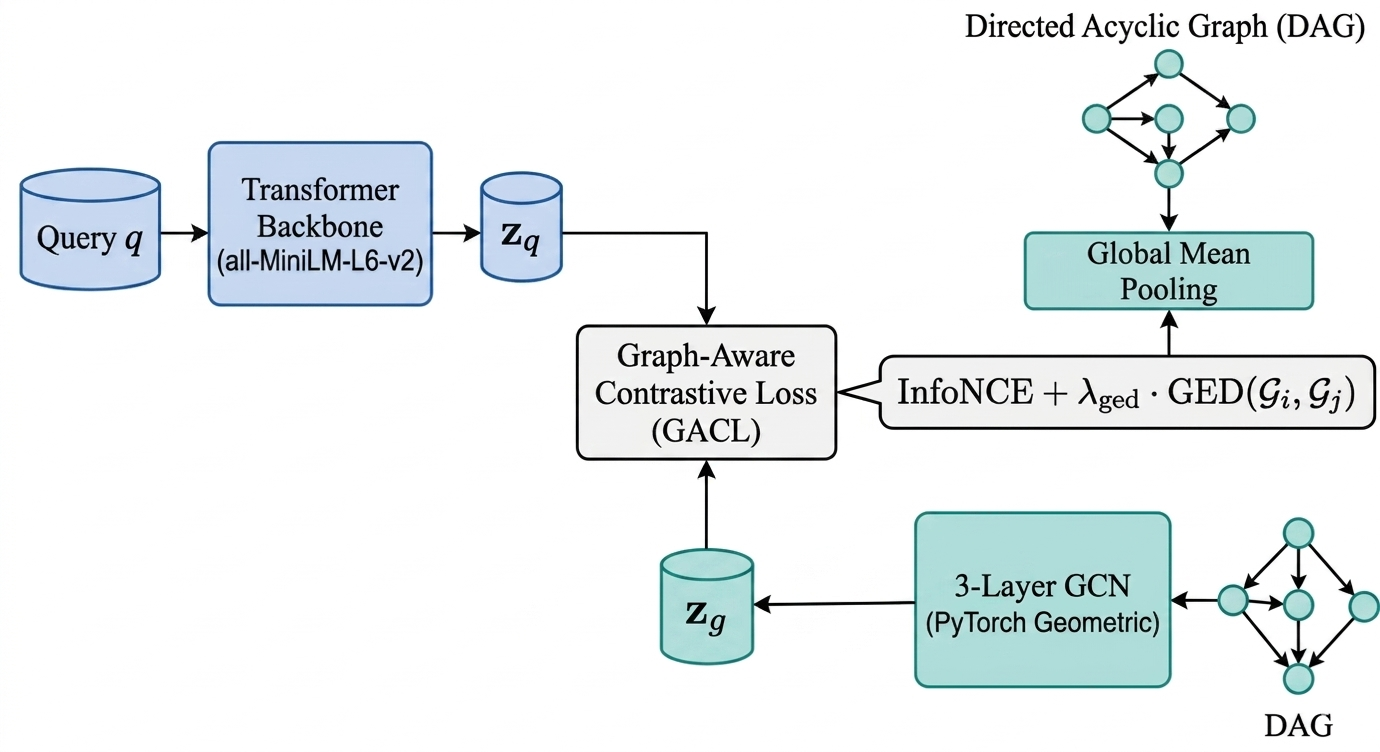
\includegraphics[width=\textwidth]{legr_arch.png}
  \caption{\textbf{Overview of the LEGR Architecture.} Our proposed dual-tower encoder maps natural language queries (Text Tower, Blue) and execution Directed Acyclic Graphs (DAG Tower, Teal) into a shared, topologically informed latent space $\mathbb{R}^d$. The training objective is regularized by the Graph-Aware Contrastive Loss (GACL), which modulates the repulsion strength based on the Graph Edit Distance (GED) between pairs.}
  \label{fig:arch}
\end{figure}

\subsection{Graph-Aware Contrastive Loss (GACL)}
LEGR is trained to align request and DAG embeddings with a symmetric contrastive objective. Given a batch of $B$ pairs $\{(q_i, \mathcal{G}_i)\}_{i=1}^B$, we form a similarity matrix $\mathbf{S}$ with entries $\mathbf{S}_{ij} = (\mathbf{z}_{q_i} \cdot \mathbf{z}_{g_j}) / \tau$, where $\tau$ is a temperature.

Standard InfoNCE implicitly treats all negatives equally. For execution graphs, this is suboptimal: many negatives share the same tool set but differ in a small number of edges, and these ``near-miss'' graphs are the ones a planner must not confuse. We therefore regularize the contrastive loss with Graph Edit Distance (GED) so that negatives with low GED are penalized more strongly.

Concretely, the total loss is:
\begin{equation}
\mathcal{L} = \frac{1}{2} \left( \text{CE}(\mathbf{S}, \mathbf{y}) + \text{CE}(\mathbf{S}^\top, \mathbf{y}) \right) + \lambda_{ged} \cdot \mathcal{L}_{ged}
\end{equation}
where $\text{CE}$ represents the standard cross-entropy loss over the similarity matrix. The structural term is:
\begin{equation}
\mathcal{L}_{ged} = \frac{1}{B} \sum_{i=1}^B -\log \frac{e^{\mathbf{S}_{ii}}}{e^{\mathbf{S}_{ii}} + \sum_{j \neq i} e^{\mathbf{S}_{ij}}(1 - \tilde{w}_{ij})}
\end{equation}
where $\tilde{w}_{ij}$ is a normalized, margin-clamped GED between $\mathcal{G}_i$ and $\mathcal{G}_j$:
\begin{equation}
\tilde{w}_{ij} = \text{clip} \left( \frac{\text{GED}(\mathcal{G}_i, \mathcal{G}_j)}{\text{ged\_scale}} - \text{margin}, 0, 1 \right)
\end{equation}
Because exact GED computation is NP-hard, we pre-compute the pairwise GED matrix for the candidate corpus $\mathcal{C}$ offline using standard approximation heuristics, ensuring this regularization adds zero overhead to the training loop. The hyperparameters $\text{ged\_scale}$ and $\text{margin}$ control the penalty threshold. This formulation preserves (and therefore strongly repels) structurally similar negatives (low GED), while down-weighting structurally distant ones. As a result, the latent space is encouraged to organize by \emph{workflow topology} rather than by tool overlap alone.



\section{Dataset and Experimental Setup}

We evaluate two questions: (i) whether \emph{Functional} supervision improves intent-to-tool routing robustness under linguistic shift, and (ii) whether LEGR can retrieve the correct \emph{execution DAG} (including edges, not just tool sets) and generalize to unseen workflow \emph{topologies}. To this end, we construct a benchmark of paired natural-language requests and \emph{ground-truth} execution graphs, with controlled topology families and stress-tested query variants.

\subsection{Execution-Graph Corpus}
We derive the tool vocabulary and natural-language intents from existing tool-use benchmarks (ToolBench \cite{qin2023toolllm} and BFCL \cite{yan2024berkeley}), and convert each example into an executable \emph{ground-truth} workflow graph $\mathcal{G}=(\mathcal{V},\mathcal{E})$. To ensure coverage of non-chain structures, we augment the corpus with template-generated DAGs that reuse the same tool library but vary only the dependency pattern. To mitigate dataset-creation bias, the topology templates and linguistic variations were generated programmatically using a fixed set of rules prior to model training, ensuring the evaluation set was not inadvertently tailored to LEGR's latent space. For example, synonym substitution was enforced via WordNet \cite{miller1995wordnet} rather than manual author selection, and graph edges were populated using strict input-output type matching between tools.

We annotate each ground-truth workflow with a \textit{Topology Family} label using simple structural heuristics. Families include \textit{Chain}, \textit{Fan-out}, \textit{Diamond} (edges $0\to1, 0\to2, 1\to3, 2\to3$), and \textit{Hourglass} (edges $0\to2, 1\to2, 2\to3, 2\to4$).

\subsection{Topology-Family Held-Out Split}
To test structural generalization (not memorization), we adopt a topology-family split rather than random shuffling. The training split contains only \textit{Chain} and \textit{Hourglass} graphs, while the \textit{Diamond} family is reserved exclusively for evaluation (\texttt{test\_topology\_heldout}). To prevent leakage, we deduplicate workflows using a hash of the labeled multiset of tool nodes and directed edges, ensuring no identical (tool, edge) signature appears in both train and test.

\subsection{Linguistic Variations}
For taxonomy-routing experiments, we evaluate under four query conditions designed to isolate common routing failures:
\begin{enumerate}
    \item \textbf{Standard:} original queries with explicit intent.
    \item \textbf{Lexical:} keyword-masked or synonym-substituted queries to reduce noun matching.
    \item \textbf{Confusable:} queries targeting sibling tools with overlapping descriptions but different action types.
    \item \textbf{Paraphrase:} syntactic rephrasings with preserved intent.
\end{enumerate}

\subsection{Baselines, Metrics, and Implementation}
We compare LEGR to sparse lexical retrieval (BM25) and dense semantic retrieval (Sentence-BERT). For execution-graph retrieval, we report Tool-Set F1, Recall@$k$, and Mean Graph Edit Distance (GED). For routing, we report end-to-end accuracy under each stress condition. LEGR uses \texttt{all-MiniLM-L6-v2} for the text tower and a 3-layer directed GNN (hidden size 256) for the graph tower, trained with $\lambda_{ged}=0.30$. Unless otherwise stated, we keep the same hyperparameters across the 15, 30, and 45-tool settings and scale only the tool vocabulary and corresponding candidate graph corpus.


\section{Experiments and Results}

In this section, we empirically validate our two core hypotheses: (1) supervising intent routing with a \emph{functional taxonomy} improves robustness against lexical variations, and (2) formulating multi-step planning as \emph{latent execution-graph retrieval} (LEGR) achieves high structural accuracy and constant-time latency, even on unseen topologies.

\subsection{Taxonomy Robustness in Intent Routing}
We first evaluate intent routing as a supervised classification task. Given a natural-language request, the router must select the correct tool branch. Table~\ref{tab:routing_results} reports the end-to-end accuracy under the four linguistic stress conditions defined in Section~4.3 using a 15-tool library. We compare two supervision schemes: a standard topic-based \emph{Semantic} taxonomy and our proposed action-based \emph{Functional} taxonomy.

\begin{table}[h]
\caption{End-to-End Routing Accuracy (\%) across various linguistic stress conditions.}
\label{tab:routing_results}
\centering
\begin{tabular}{@{}lcccccccc@{}}
\toprule
& \multicolumn{4}{c}{\textbf{GPT-OSS}} & \multicolumn{4}{c}{\textbf{Llama 3.2}} \\
\cmidrule(lr){2-5} \cmidrule(lr){6-9}
Taxonomy & Std. & Lex. & Conf. & Para. & Std. & Lex. & Conf. & Para. \\
\midrule
Topic-based & 78.3 & 68.1 & 62.7 & 78.0 & 70.0 & 43.3 & 43.3 & 64.9 \\
\textbf{Functional} & \textbf{93.3} & \textbf{75.6} & \textbf{68.0} & \textbf{90.6} & \textbf{83.8} & \textbf{61.8} & \textbf{55.3} & \textbf{79.8} \\
\bottomrule
\end{tabular}
\end{table}

As shown in Table~\ref{tab:routing_results}, the Functional taxonomy consistently outperforms the Topic-based taxonomy across all regimes and both LLM routers. The most significant improvements are observed under conditions where topic nouns are unreliable. For instance, under the \textit{Lexical} stress condition (keyword masking and synonym substitution), Llama 3.2 accuracy improves by 18.5 absolute percentage points (43.3\% to 61.8\%), and GPT-OSS improves by 7.5 points (68.1\% to 75.6\%). Similarly, under the \textit{Confusable} regime (sibling tools with overlapping descriptions but distinct action types), both models demonstrate enhanced robustness. These results substantiate the hypothesis that grouping tools by action type (read, write, orchestrate) provides a more reliable supervision signal than topical clustering, mitigating the router's tendency to overfit to surface vocabulary.

\subsection{Execution-Graph Retrieval and Efficiency}
Next, we evaluate LEGR's ability to retrieve the correct execution DAG compared to lexical (BM25) and dense (S-BERT) retrieval baselines, as well as state-of-the-art autoregressive generation (Llama 3.2 and GPT-OSS). Table~\ref{tab:retrieval_metrics} presents the structural alignment and inference latency on the \textit{test\_topology\_heldout} split (15-tool setting), which exclusively contains Diamond topologies unseen during training.

\begin{table}[h]
\caption{Structural Retrieval and Latent Alignment Metrics on Held-Out Topologies (15 Tools).}
\label{tab:retrieval_metrics}
\centering
\small
\begin{tabular}{@{}lccccc@{}}
\toprule
\textbf{Model} & \textbf{Tool-Set F1} & \textbf{Recall@1} & \textbf{Mean GED $\downarrow$} & \textbf{Latency (ms)} & \textbf{Speedup} \\
\midrule
BM25             & 0.223 & 0.014 & 6.030 & \textbf{0.41} & $10.7\times$ \\
S-BERT           & 0.610 & 0.302 & 4.618 & 9.10 & $0.48\times$ \\
\midrule
LEGR (no GED)    & 0.984 & 0.944 & 0.221 & 4.19 & $1.05\times$ \\
\textbf{LEGR (with GED)} & \textbf{0.995} & \textbf{0.963} & \textbf{0.111} & 4.39 & $1\times$ \\
\midrule
Llama 3.2 (Gen)  & 0.690 & 0.690 & 4.532 & 1,760.0 & $0.0025\times$ \\
GPT-OSS (Gen)    & 0.961 & 0.961 & 1.590 & 2,742.0 & $0.0016\times$ \\
\bottomrule
\end{tabular}
\end{table}

\textbf{Structural Generalization.} LEGR demonstrates strong zero-shot structural generalization, achieving a Recall@1 of 0.963 and a Tool-Set F1 of 0.995. In contrast, standard S-BERT struggles to differentiate between topologically distinct graphs that share similar tool sets, yielding a Recall@1 of 0.302. The inclusion of the Graph-Aware Contrastive Loss (GACL) with GED regularization is critical for this performance, reducing the Mean GED by 50\% (0.221 to 0.111) compared to the unregularized LEGR variant.

\textbf{Inference Efficiency.} By replacing sequential token generation with a single dense retrieval step, LEGR achieves a mean inference latency of 4.39\,ms. This represents a substantial speedup over autoregressive baselines: approximately $401\times$ faster than Llama 3.2 (1,760\,ms) and $625\times$ faster than GPT-OSS (2,742\,ms). Furthermore, Table~\ref{tab:retrieval_metrics} reveals a severe latency-accuracy trade-off in the baselines. The only baseline faster than LEGR is BM25 (0.41\,ms), but its structural accuracy is near zero (Recall@1 = 0.014). Conversely, the only baseline approaching LEGR's tool-set accuracy is GPT-OSS, but it requires nearly 3 seconds per query. LEGR is the only method that breaks this Pareto frontier, delivering state-of-the-art structural accuracy at millisecond latencies. This constant-time inference profile is particularly advantageous for real-time agentic systems where planning latency often dominates end-to-end responsiveness.

\subsection{Scalability to Larger Tool Libraries}
To assess performance as the action space expands, we scale the tool vocabulary to 30 and 45 tools and evaluate on the held-out Diamond topologies. Table~\ref{tab:scalability} summarizes the retrieval performance across these scales.

\begin{table}[h]
\caption{Scalability of LEGR and baselines across 15, 30, and 45 tools on held-out topologies. LEGR achieves Recall@5 = 1.0 at every scale. $\dagger$~Generative models produce a single plan; Recall@1 is reported as Tool-Set F1.}
\label{tab:scalability}
\centering
\small
\begin{tabular}{@{}llcccc@{}}
\toprule
\textbf{Tools} & \textbf{Model} & \textbf{Tool-Set F1} & \textbf{Recall@1} & \textbf{Recall@5} & \textbf{Mean GED $\downarrow$} \\
\midrule
\multirow{5}{*}{15}
  & BM25                          & 0.223 & 0.014 & 0.068 & 6.030 \\
  & S-BERT                        & 0.610 & 0.302 & 0.694 & 4.618 \\
  & Llama 3.2 (Gen)$^\dagger$     & 0.690 & 0.690 & —     & 4.532 \\
  & GPT-OSS (Gen)$^\dagger$       & 0.961 & 0.961 & —     & 1.590 \\
  & \textbf{LEGR (Ours)}          & \textbf{0.995} & \textbf{0.963} & \textbf{1.000} & \textbf{0.111} \\
\midrule
\multirow{5}{*}{30}
  & BM25                          & 0.1508 & 0.012 & 0.056 & 6.358 \\
  & S-BERT                        & 0.531 & 0.316 & 0.663 & 3.811 \\
  & Llama 3.2 (Gen)$^\dagger$     & 0.602 & 0.602 & —     & 6.903 \\
  & GPT-OSS (Gen)$^\dagger$       & 0.963 & 0.963 & —     & 1.304 \\
  & \textbf{LEGR (Ours)}          & \textbf{0.997} & \textbf{0.989} & \textbf{1.000} & \textbf{0.038} \\
\midrule
\multirow{5}{*}{45}
  & BM25                          & 0.106 & 0.010 & 0.048 & 9.884 \\
  & S-BERT                        & 0.621 & 0.463 & 0.789 & 3.686 \\
  & Llama 3.2 (Gen)$^\dagger$     & 0.578 & 0.578 & —     & 7.325 \\
  & GPT-OSS (Gen)$^\dagger$       & 0.959 & 0.959 & —     & 1.578 \\
  & \textbf{LEGR (Ours)}          & \textbf{0.987} & \textbf{0.975} & \textbf{1.000} & \textbf{0.134} \\
\bottomrule
\end{tabular}
\end{table}

\begin{figure}[htbp]
    \centering
    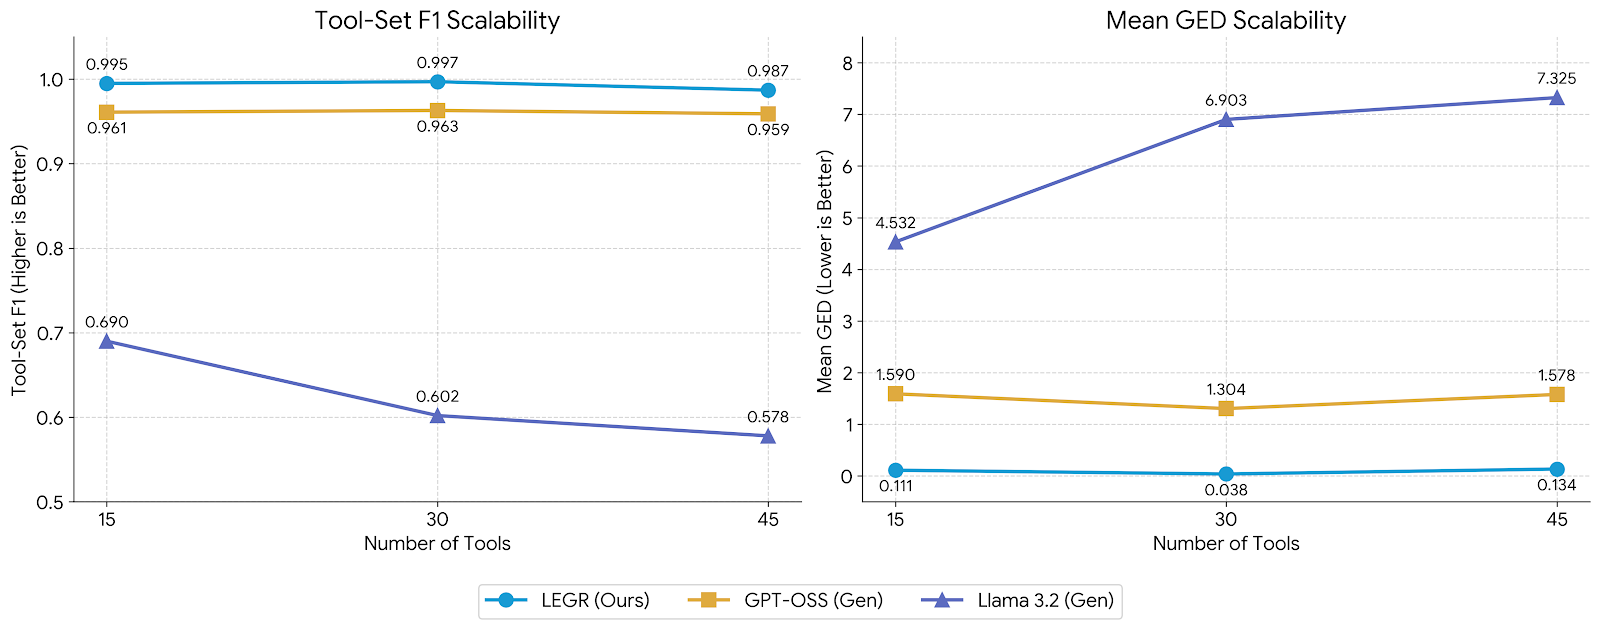
\includegraphics[width=\textwidth]{tool_scale.png}
    \caption{\textbf{Scalability of LEGR compared to Generative Baselines.} Performance across 15, 30, and 45 tools for LEGR, GPT-OSS, and Llama 3.2. \textbf{Left:} Tool-Set F1 score (higher is better). \textbf{Right:} Mean Graph Edit Distance (GED, lower is better). LEGR maintains near-perfect set matching and minimal structural error across all scales. In contrast, Llama 3.2 exhibits a marked degradation in both F1 and GED as the tool space expands.}
    \label{fig:scalability_metrics}
\end{figure}

\textbf{Retrieval Robustness.} LEGR maintains high retrieval accuracy at scale, sustaining a Recall@5 of 1.0 and a Tool-Set F1 above 0.987 across all tool counts. The Mean GED remains below 0.135, indicating that the latent space effectively preserves topological structure even as the candidate corpus grows and the action space widens.

\textbf{Baseline Degradation.} In contrast, baseline methods exhibit performance degradation as the vocabulary expands. Lexical retrieval (BM25) shows a marked increase in Mean GED (from 6.030 at 15 tools to 9.884 at 45 tools) and a drop in Tool-Set F1, highlighting the limitations of keyword matching for complex routing. Autoregressive generation also struggles; Llama 3.2's Tool-Set F1 decreases monotonically (0.690 to 0.578), and its Mean GED worsens (4.532 to 7.325), reflecting the compounding difficulty of synthesizing valid multi-tool plans over a broader action space. While GPT-OSS maintains a stable Tool-Set F1, its structural error (Mean GED) remains an order of magnitude higher than LEGR's. Notably, GPT-OSS's Recall@1 perfectly matches its Tool-Set F1 across all scales (0.961, 0.963, 0.959). This indicates a critical failure mode of autoregressive planners: when GPT-OSS selects the correct set of tools, it almost always hallucinates the wrong dependency edges, resulting in a correct tool set but a topologically invalid DAG. LEGR, by retrieving pre-validated graphs, avoids this structural hallucination entirely.

\textbf{Taxonomy Granularity at Scale.} While LEGR scales robustly for execution-graph retrieval, we observed that the three-way Functional taxonomy (read, write, orchestrate) used for intent routing becomes under-specified at 30 and 45 tools. As the vocabulary grows, multiple tools share the same top-level action type but differ in secondary constraints (e.g., entity scope or permissions), leading to within-branch confusion. Addressing this requires a hierarchical taxonomy or a learned continuous router, which we identify as a direction for future work.

\subsection{Parameter Footprint and Computational Cost}
Finally, we contextualize LEGR's performance in terms of model size. Table~\ref{tab:model_size} compares the parameter counts, structural accuracy, and latency of the evaluated methods.

\begin{table}[h]
\caption{Efficiency Comparison: Parameter Count vs. Structural Accuracy and Latency. LEGR achieves significantly lower graph edit distance (GED) errors than a 120B parameter autoregressive model while operating over $600\times$ faster.}
\label{tab:model_size}
\centering
\small
\begin{tabular}{@{}llccc@{}}
\toprule
\textbf{Model} & \textbf{Architecture} & \textbf{Parameters} & \textbf{Mean GED $\downarrow$} & \textbf{Latency (ms) $\downarrow$} \\
\midrule
GPT-OSS 120B & Autoregressive LLM & $\approx$ 120.0 Billion & 1.590 & 2,742.00 \\
Llama 3.2    & Autoregressive LLM & $\approx$ 8.0 Billion   & 4.532 & 1,760.00 \\
\midrule
BM25         & Lexical Retrieval  & 0                       & 6.030 & \textbf{0.41} \\
S-BERT       & Dense Retrieval    & $\approx$ 22.7 Million  & 4.618 & 9.10 \\
\textbf{LEGR (Ours)} & \textbf{S-BERT + 3-Layer GNN} & \textbf{$\approx$ 23.5 Million} & \textbf{0.111} & 4.39 \\
\bottomrule
\end{tabular}
\end{table}

LEGR achieves state-of-the-art structural alignment with a total footprint of approximately 23.5 million parameters (a 22.7M parameter text backbone and a lightweight 3-layer GNN). Compared to the 120B parameter GPT-OSS baseline, LEGR offers a substantial reduction in model size (by a factor of $\sim 5,100\times$) and mean inference latency (from 2,742\,ms to 4.39\,ms), while simultaneously reducing the Mean GED from 1.590 to 0.111. These results demonstrate that accurate multi-tool orchestration does not strictly require massive autoregressive models; rather, it can be efficiently solved via topology-aware retrieval in a properly regularized latent space.

\section{Ablation Study and Sensitivity Analysis}

To isolate the contributions of specific architectural and training components to LEGR's performance, we conduct ablation and sensitivity analyses on the \textit{test\_topology\_heldout} split.

\subsection{Ablation of GED Regularization}
We first evaluate the necessity of the Graph-Aware Contrastive Loss (GACL) by comparing the full LEGR model ($\lambda_{ged}=0.30$) against an unregularized variant ($\lambda_{ged}=0$), which reduces the training objective to standard InfoNCE. As shown in Table~\ref{tab:retrieval_metrics}, while both variants successfully identify the correct set of tools (Tool-Set F1 of 0.995 vs.\ 0.984), the unregularized model exhibits a $2.0\times$ degradation in structural alignment, with the Mean GED increasing from 0.111 to 0.221. This divergence demonstrates that standard contrastive training is sufficient for semantic tool retrieval but insufficient for topological planning. The GED-weighted denominator is strictly required to internalize the directed edges of the execution DAG, effectively converting a tool-set retriever into a true execution-graph retriever.

\subsection{Sensitivity to Tool Vocabulary Scale}
To assess LEGR's robustness to expanding action spaces, we analyze its sensitivity to tool vocabulary sizes of 15, 30, and 45 tools (detailed in Section~5.3). Across all three configurations, LEGR sustains a saturated Recall@5 of 1.0 on unseen Diamond topologies. Interestingly, the Mean GED exhibits a non-monotonic trend: it decreases from 0.111 (15 tools) to 0.038 (30 tools) before rising to 0.134 (45 tools). We attribute this behavior to the interplay between training corpus diversity and inference branching factor. Expanding from 15 to 30 tools introduces greater structural diversity during training, which tightens the latent representation and improves alignment. However, scaling to 45 tools significantly widens the action space, introducing a higher density of near-isomorphic Diamond graphs that compete within the top-5 ranking. 

While this non-monotonicity suggests that scaling to hundreds of tools increases the density of topologically similar "near-miss" graphs, it is crucial to contextualize this error. For context, large production agentic systems such as Claude Code currently operate with approximately 20 tools \cite{claude_code_tools}, meaning our 45-tool evaluation already stress-tests LEGR well beyond typical deployment scales. Even at its peak (GED of 0.134 at 45 tools), LEGR's structural error remains an order of magnitude lower than the best-performing generative baseline (GPT-OSS, GED of 1.578) and vastly superior to standard dense retrieval baselines. This confirms that while future work may require harder negative mining to maintain separation at enterprise scales (e.g., $10^3+$ tools), LEGR's latent space remains highly topologically coherent and achieves state-of-the-art structural accuracy within current operational tool limits.

\section{Qualitative Analysis}

\subsection{Mitigating Topic Confusion}
A qualitative review of routing failures under the Topic-based taxonomy reveals a systemic vulnerability to lexical overlap. For example, the router frequently misclassified "State Modification" intents into "Data Retrieval" branches when sibling tools shared prominent topic nouns (e.g., \texttt{Update\_User\_Profile} versus \texttt{Get\_User\_Profile}). By reorganizing the label space around action types, the Functional taxonomy effectively eliminates this failure mode. It forces the router to attend to the verb-phrase action (the intended action) rather than the noun-phrase entity (the topic subject), thereby resolving the topic confusion gap.

\begin{figure}[t]
  \centering
  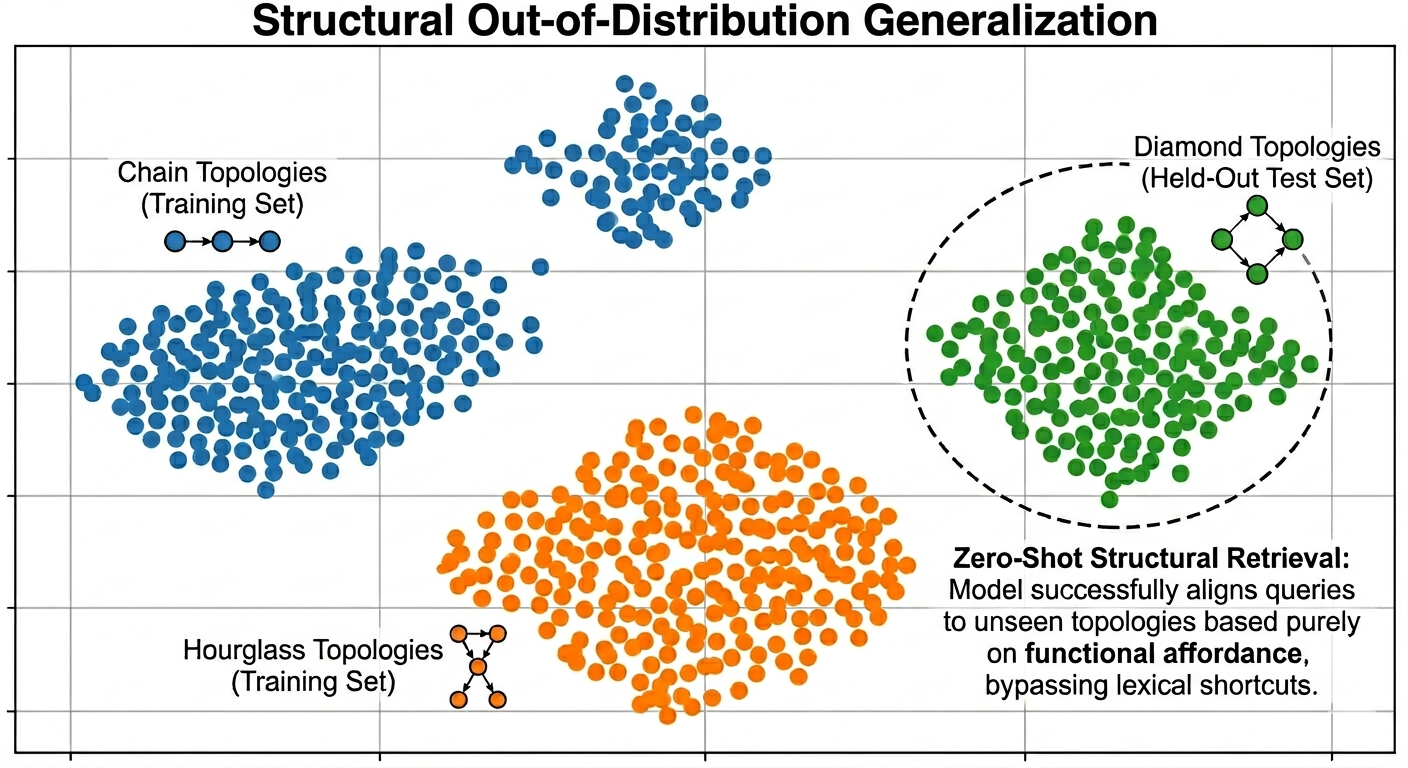
\includegraphics[width=\textwidth]{struct.png}
  \caption{\textbf{Latent Space Topology Visualization.} A 2D projection (t-SNE) of the shared latent space $\mathbb{R}^d$. While the model is trained only on Chain (Blue) and Hourglass (Orange) topologies, it successfully clusters Held-Out Diamond topologies (Green) in a distinct, coherent region. This demonstrates \textbf{Structural Zero-Shot Generalization}, where the model maps natural language intent to complex, unseen execution structures based on functional action type rather than lexical rote-learning.}
  \label{fig:latent_viz}
\end{figure}

\subsection{Structural Zero-Shot Generalization}
LEGR's ability to accurately retrieve "Diamond" topologies, despite only being exposed to "Chain" and "Hourglass" structures during training, demonstrates that the GNN encoder learns a generalizable representation of dependency flow rather than memorizing specific training graphs. Figure~\ref{fig:latent_viz} visualizes a t-SNE projection of the shared latent space, illustrating a clean separation of the held-out Diamond topologies from the training clusters. 

The current topological organization is a direct consequence of the GED-weighted denominator in the GACL objective, which prevents the latent space from collapsing along superficial lexical axes. By down-weighting structurally distant negatives during contrastive training, the loss structures the latent space according to underlying workflow topology. This capability represents a critical step toward zero-shot planning, enabling agents to orchestrate novel workflow structures provided the functional requirements are understood.


\section{Discussion and Conclusion}

In this work, we address two fundamental bottlenecks in agentic intent routing: the fragility of topic-based tool selection and the computational latency of autoregressive multi-step planning. Our findings challenge the prevailing assumptions that tool libraries should mirror human topics and that workflow planning requires token-by-token generation.

\textbf{Revisiting Routing Supervision.} First, we demonstrate that organizing tools by \emph{action type} (the Functional Taxonomy) provides a significantly more robust supervision signal than traditional topical clustering. By forcing the router to attend to operational intent (e.g., read vs.\ write) rather than topical keywords, we achieved up to an 18.5 percentage point improvement in routing accuracy under lexical variations. This confirms that the brittleness of current routing systems stems primarily from a \textit{representation mismatch}: when supervision relies on topic nouns, models inevitably overfit to surface lexical cues, failing when those cues are perturbed or omitted.

\textbf{Retrieval as Planning.} Second, we introduced Latent Execution-Graph Retrieval (LEGR), which reframes multi-tool orchestration as a cross-modal retrieval task. Optimized via our Graph-Aware Contrastive Loss (GACL), LEGR internalizes workflow topology, achieving perfect Recall@5 on unseen Diamond topologies with a Mean GED of 0.111. Crucially, LEGR decouples planning complexity from inference latency. By replacing sequential decoding with a single dense retrieval step, LEGR operates in constant time (4.39\,ms), an over $600\times$ speedup compared to a 120B-parameter LLM baseline, while requiring only $\sim$23.5M parameters. Furthermore, these advantages compound at scale: as the tool vocabulary expands to 45 tools, LEGR sustains near-perfect structural alignment while autoregressive baselines suffer from severe structural hallucinations.

\textbf{Implications for Agentic Systems.} The implications of these results are twofold. Operationally, LEGR's sub-5\,ms latency and minimal parameter footprint enable complex agentic orchestration to run natively on edge devices or within high-throughput microservices, environments where multi-second LLM generation is prohibitive. Architecturally, the success of GACL suggests that graph-theoretic regularizers are essential for aligning natural language with executable code structures, paving the way for more reliable neuro-symbolic systems.

\textbf{Limitations.} We note three primary limitations. First, while the three-branch Functional taxonomy is effective at 15 tools, it becomes under-specified at larger scales (30--45 tools), where intra-branch sibling collisions emerge. Second, our zero-shot evaluation isolates a single structural family (Diamond DAGs). While LEGR successfully interpolates this structure, it remains untested on workflows with highly dynamic, data-dependent control flow where the topology cannot be statically bounded ahead of time. Third, LEGR currently retrieves from a precomputed, static DAG corpus, limiting its adaptability to runtime tool additions or entirely novel, unindexed workflows.

\textbf{Future Work.} These limitations suggest clear directions for future research. Developing a learned, hierarchical action router could resolve the taxonomy overlap issue at scale. Additionally, extending LEGR to support dynamic, runtime-generated graphs (perhaps by hybridizing LEGR with lightweight autoregressive mechanisms) would bridge the gap between retrieval-based efficiency and open-world adaptability for unbounded branching. Finally, LEGR's constant-time inference profile makes it an ideal candidate for multi-agent swarms, where millisecond-level routing is critical for coordinating dozens of concurrent agents.

\textbf{Conclusion.} Ultimately, our results establish that reliable multi-tool orchestration does not require massive autoregressive models. By aligning supervision with action types and offloading planning to topology-aware latent retrieval, we can achieve highly accurate, structurally sound, and real-time agentic routing at a fraction of the traditional computational cost.

\section*{Declaration of LLM Usage}
The authors used Claude 4.7 and Gemini 1.5 Pro for LaTeX formatting, structural organization, and prose refinement. The core methodology, loss function derivation, and experimental execution were developed by the authors.


\nocite{*}

\medskip
\small
\bibliographystyle{unsrt}
\bibliography{references}


\end{document}
